\section{3D exploration strategies}

\begin{figure}[t!]
	\centering
	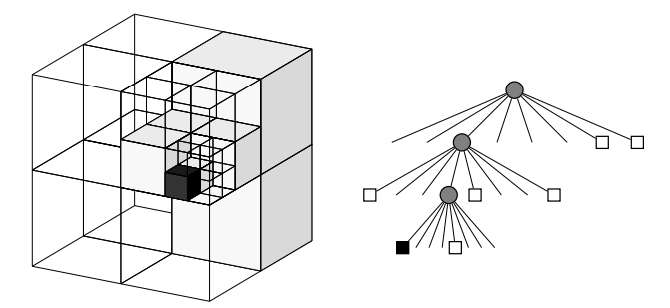
\includegraphics[width=1.0\columnwidth]{./pictures/octomap.png}	
	\caption{Illustration of the octree data-structure. Left: Example of an octree storing free voxels (shaded white) and occupied voxels (black). Right: The corresponding tree representation (Source \cite{Wurm2012}).}
	\label{fig:octomap}
\end{figure}

\begin{figure}[t!]
	\centering
	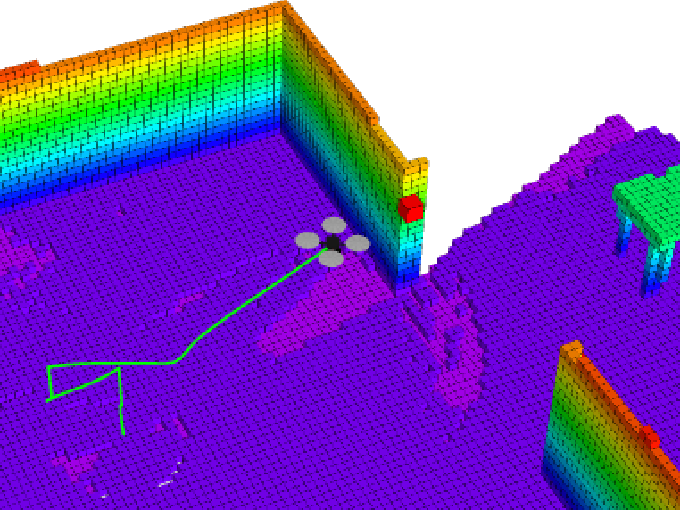
\includegraphics[width=1.0\columnwidth]{./pictures/octomap_and_drone.png}	
	\caption{An unmanned aerial vehicle (UAV) exploration in 3D environment. The colored voxels are 3D OctoMap representation and the green lines show the exploration trajectory (Source \cite{Wang2019}).}
	\label{fig:octomapanddrone}
\end{figure}

When robots autonomously navigate in a three-dimensional space, they need a model of the environment that defines regions which are safe to traverse. An approach in \cite{Wurm2012} presented \textit{OctoMap} framework which models obstacles as well as free space. It discretizes the environment by dividing it into equally-sized cubic volumes called \textit{voxels}. The approach then estimates the probability of each voxel to be occupied and maintains data in a tree-based representation that allocates memory only for those parts of the model that carry information about the environment. 
An octree is a tree-based data structure that represents the 3D space by recursively subdividing the corresponding volume into eight sub-volumes until a given minimum cube size is reached. The relation between the volumes and the tree is illustrated in Fig. \ref{fig:octomap}. A majority of the strategies use OctoMap in order to navigate through 3D space and visualize environment.

In contrast to 2D exploration and mapping strategies, mapping of large environments in 3D requires high memory and computational consumptions. In 3D as well as in 2D space, exploration can be accomplished using a single robot or multiple robots.

\subsection{A single robot exploration}  
Different autonomous 3D exploration strategies that use a single robot are presented in the following text.

In \cite{Joho2007}, Joho et al. presented an exploration strategy that extends the known 2D exploration strategies into the 3D space. Mapping is done using multi-level surface maps while a cost function takes
into account an expected information gain and a travel cost. 
Bachrach et
al. \cite{Bachrach2009} presented a solution for enabling a quadrotor helicopter to autonomously explore and map unstructured indoor environments. Authors used a 2D frontier-based exploration algorithm and set a fixed altitude for the helicopter during exploration.  

Dornhege and Kleiner \cite{Dornhege2013} used a frontier based method extended to 3D exploration. This method requires high computational effort and operating environment is limited to small workspaces. On the other hand, Maurovic et al. \cite{Maurovic2014} presented a 3D exploration strategy for a mobile robot equipped with a 3D laser scanner. This strategy ensures an online room detection algorithm focused on the room-by-room exploration keeping the memory and computational requirements low.

Next-best-view approach in the process of building 3D model of a real object used without any a priori information about the environment was described in \cite{VasquezGomez2014}. The algorithm determines each view to reconstruct an arbitrary object. Furthermore, authors proposed a method to deal with the uncertainty in sensor positioning.
Next-best-view approach for 3D exploration was presented by Bircher et. al. \cite{Bircher2016}. Authors presented a novel path planning algorithm for the autonomous exploration of an unknown area. The proposed planner finds the best branch in an online computed tree. The quality of the branch is determined by the amount of unmapped space that can be explored. The planner is capable of running online, onboard a robot with limited resources.

Baiming et al. \cite{Baiming2018} presented a new target points based trajectory planning algorithm to explore unknown space. The proposed method progressively plans long-term target point, intermediate target point, local target points, and local trajectory within real time constraint. By tracking the trajectory, robot can efficiently explore the unknown space while avoiding obstacles.

Continuous cells are gathered into clusters and representative cells are chosen for each cluster. An evaluation function is used to choose the best representative cell and only state-changed space in the 3D map is processed in each iteration.
Authors in \cite{Senarathne2016} presented an alternative approach to 3D exploration based on surface frontier voxels. The strategy focuses on seeking the expansion of mapped surfaces, instead of reducing unmapped voxels. 

Wang et al. \cite{Wang2018} studied the problem of autonomous exploration in unknown indoor environments using mutual information to evaluate the information the robot would get at a certain location. Authors proposed a sampling method that can get random sensing patches in free space. In order to to collect information with true values, each sensing patch is extended to informative locations. They combined it with Gaussian Markov Random Fields (GMRF) to model the distribution of mutual information in environment.  Authors also proposed a utility function that can balance the path cost and the information gain the robot would collect.


\subsection{Multi-robot exploration}

In this section multi-robot 3D exploration strategies are presented. A collaboration between robots plays an important role in these strategies, for instance, sharing information about frontier points, sharing the local maps of each robot to others to avoid many robots go on same paths in different times, to name a few.

Priyasad et al. \cite{Priyasad2018} presented a point cloud based algorithm which can be used in a situation where the prior knowledge of the environment is highly inaccurate. The algorithm uses depth images to get a local map, which is expanded by searching for uncharted areas picking the next best
location to explore using a breadth first approach given a set of
constraints. The proposed algorithm exploits the maps in the 3D
space allowing the navigation system to perform effectively in uneven terrains. 

Zhu et al. \cite{Zhu2015} developed a vision-based tool that performs autonomous exploration using a MAV equipped with 3D sensors. A real time frontier based exploration strategy is used to build maps that are stored in the OctoMap format (Fig. \ref{fig:octomapanddrone}).

Vutetakis in \cite{Vutetakis2019} proposed a novel strategy for inspecting critical infrastructure autonomously using Micro Aerial Vehicles (MAVs). In order to facilitate autonomous inspection capabilities, this strategy addresses the problem of autonomous MAVs exploration and coverage of an unknown structure to acquire the spatial information necessary for the development of a high-fidelity 3D model of the structure. Key to this problem is to not only cover the entire structure, but also to minimize accumulative data errors during the exploration through direct planning of loop closures. 

Rocha et al. \cite{Rocha2005} dealt with 3D mapping by multiple robots using cubic cells for information storage. Authors presented a technique which is used for frontier-based exploration. At the beginning of the exploration an initial map is given to the robot, the robots update old map by new set of information obtained through sensing and share their useful information with other robots. The process is repeated until the whole area is explored and mapped.


\begin{figure}[t!]
	\centering
	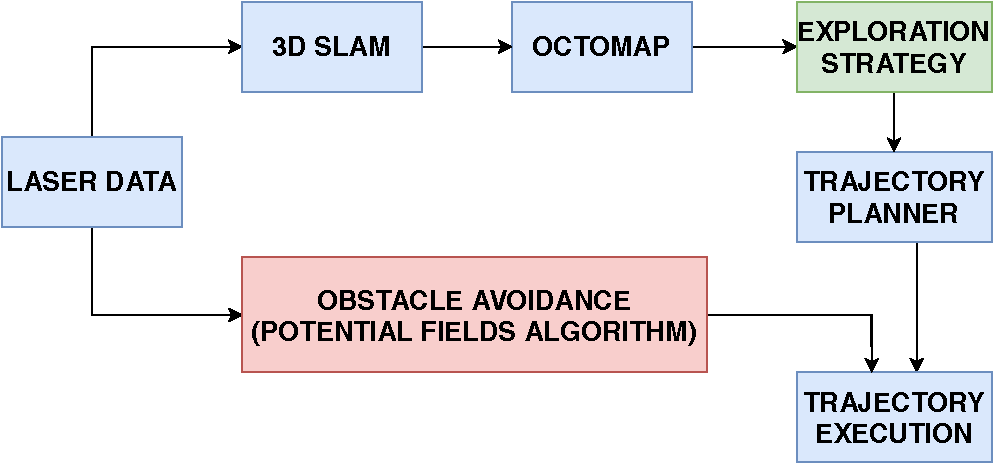
\includegraphics[width=1.0\columnwidth]{./pictures/3D_strategy.pdf}	
	\caption{Diagram of the implemented 3D exploration strategy.}
	\label{fig:3D_strategy}
\end{figure}

The 3D exploration problem using aerial vehicles within limited flight endurance was addressed by Wang et al. \cite{Wang2019}. Authors proposed an information potential field based method considering both the traveled cost and information-gain. The next-best-view point is chosen based on a multi-objective function which considers information of several candidate regions and the traveled path cost. The selected goal
attracts the robot while known obstacles form the repulsive
force repel the robot.

There are many algorithms to implement autonomous exploration as we described in the text above. Most of the algorithms are dependent on prior knowledge of the environment and apriori maps. Although they are effective in some scenarios, these algorithms fail to perform when the environment has been subjected to changes that might invalidate the prior map. There are also algorithms implemented to deal with single robot exploration and mapping. Motivated by mentioned facts, we studied the problem of autonomous multi-robot building exploration with purpose of fire detection.

Overall schematic diagram of the implemented exploration and mapping process is shown in Fig \ref{fig:3D_strategy}. Besides the localization and mapping of an unknown area and exploration strategy, an OctoMap generation and trajectory execution are also important modules of the outdoor exploration. OctoMap is created from Google Cartographer's \textit{submap point cloud}. Cartographer primarily consists of two subsystems, global SLAM and local SLAM. Local SLAM is used to generate submaps of the region and global SLAM is used to tie the submaps together as consistently as possible. The result of the exploration strategy is a target point that represents an input to trajectory planner. Currently, target points are generated from the Global Positioning System (GPS) location of the building as shown in Fig. \ref{fig:building}. Then the trajectory planner generate trajectory using OctoMap and a UAV executes it (Fig. \ref{fig:rviz_gazebo}).

\begin{figure}[t!]
	\centering
	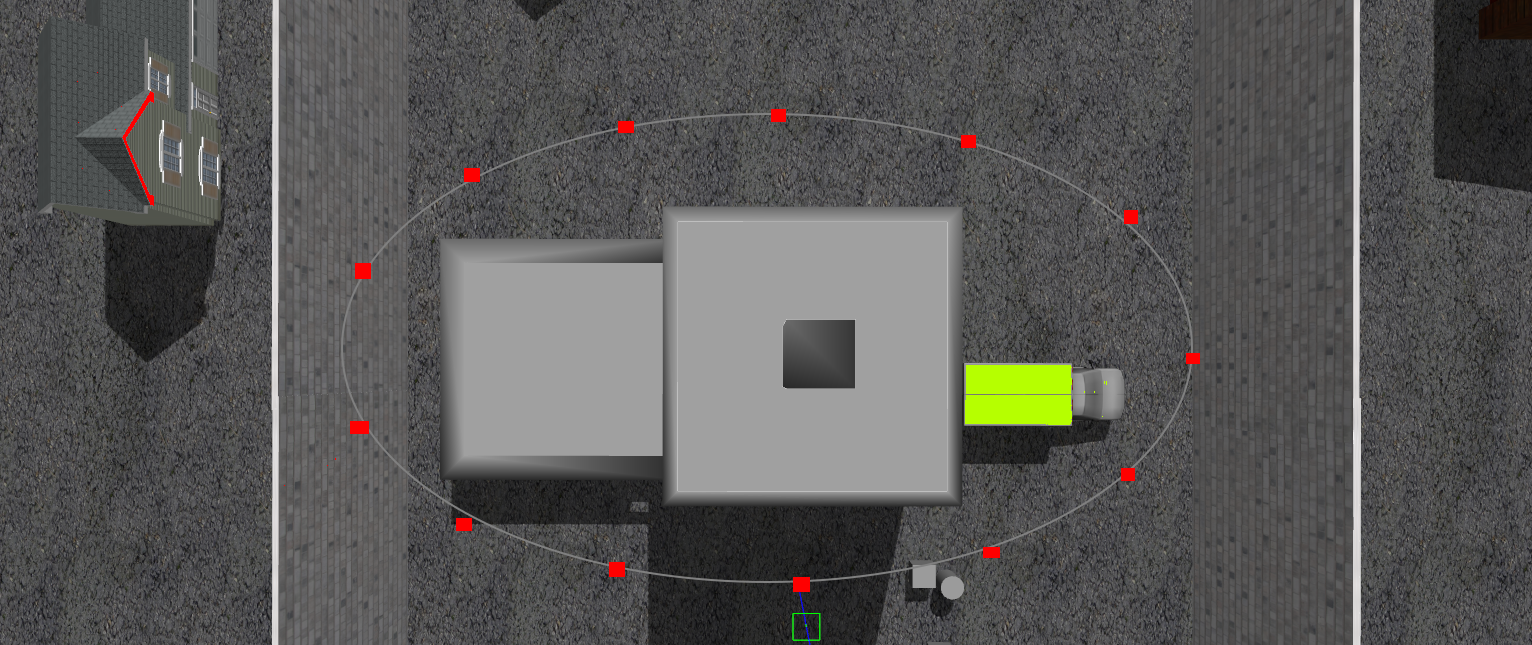
\includegraphics[width=1.0\columnwidth]{./pictures/building.png}	
	\caption{Ellipse-shaped target points generated from the GPS location of the building center.}
	\label{fig:building}
\end{figure}

An obstacle avoidance algorithm based on potential fields is also considered in our work. Due to the fact that a map is on-line created and the trajectory planner generates trajectory without replanning during the execution, generated trajectory points need to be locally validated and if necessary corrected. Hence, we send robot laser data to a potential fields obstacle avoidance algorithm. In case a robot is executing the trajectory and a current robot position is too close to the static obstacle or dynamic obstacle is detected, our obstacle avoidance algorithm is activated and generated trajectory is corrected.  

